% one_pager.tex — 1-page technical note companion to
% github.com/rajo69/AI-Accountant-with-Reinforcement-Learning-Routing
% Compile: pdflatex paper/one_pager.tex
\documentclass[10pt,a4paper]{article}

\usepackage[margin=1.8cm]{geometry}
\usepackage[T1]{fontenc}
\usepackage{lmodern}
\usepackage{microtype}
\usepackage{graphicx}
% Search for figures under both possible working directories so `pdflatex
% paper/one_pager.tex` works whether invoked from the repo root or from paper/.
\graphicspath{{experiments/results/figures/}{../experiments/results/figures/}}
\usepackage{booktabs}
\usepackage{array}
\usepackage[hidelinks]{hyperref}
\usepackage{titling}
\usepackage{enumitem}

\setlength{\droptitle}{-1.6cm}
\setlength{\parskip}{3pt}
\setlength{\parindent}{0pt}
\renewcommand{\arraystretch}{1.05}
\pagestyle{empty}

\title{\vspace{-0.6cm}\textbf{Learned Routing Under Uncalibrated LLM Confidence:\\a PPO Case Study on a Production Accounting Pipeline}}
\author{Rajarshi Nandi \\ \small \texttt{rajarshin264@gmail.com} \quad \href{https://github.com/rajo69/AI-Accountant-with-Reinforcement-Learning-Routing}{github.com/rajo69/\ldots-Routing}}
\date{\vspace{-0.4cm}\small April 2026}

\begin{document}
\maketitle
\vspace{-0.6cm}

\textbf{Problem.}
Production agentic pipelines increasingly rely on fixed confidence thresholds to
decide when an LLM-based component may act autonomously versus escalate to a human.
These thresholds (e.g.\ \texttt{conf > 0.85 $\Rightarrow$ auto-approve}) are hand-tuned
and do not adapt to input difficulty, stakes, or operator load. Confidence-gated
autonomy is a core unsolved problem for production deployments of agentic AI.

\textbf{Question.}
Can a lightweight PPO policy, observing the same confidence score plus a
handful of transaction features, outperform the hand-tuned threshold routing of a
production LLM agent on a real-world pipeline?

\textbf{Setup.}
The parent system is an AI bookkeeping assistant for UK accountants. A
\textit{CategoriserAgent} (Claude Haiku via Instructor) assigns a category and a
confidence score to each Xero bank transaction; a hand-tuned router then picks
one of three actions: \textsc{auto-approve}, \textsc{surface-for-review}, or
\textsc{reject-for-manual}. We formalise this as a Gymnasium MDP, generate 882
synthetic transactions (stratified 80/20, real Claude confidence scores) from 50
labelled seeds, and train three PPO variants (Stable-Baselines3~2.7.1, 100k
steps, seed=42) corresponding to three deployment priorities: a typical firm (A),
a workload-weighted high-volume firm (B), and a compliance-critical setting (C)
with a 5$\times$ penalty on silent auto-approval errors.

\textbf{Results} (held-out $n{=}177$; Wilson~95\%~CIs; two-proportion~$z$-tests).

\begin{center}
\small
\begin{tabular}{lcccc}
\toprule
Metric & Baseline & PPO (A/B/C) & $p$ \\
\midrule
Routing accuracy (all 177)     & 66.7\% [59.4, 73.2] & 63.3\% [56.0, 70.0] & 0.50 \\
Auto-approval precision        & 72.6\% [63.7, 79.9] & 77.8\% [67.6, 85.5] & 0.41 \\
Auto-approval error rate       & 27.4\% [20.1, 36.3] & 22.2\% [14.5, 32.4] & 0.41 \\
\textbf{Auto-approval rate}    & \textbf{63.8\% [56.5, 70.6]} & \textbf{45.8\% [38.6, 53.1]} & \textbf{0.001} \\
\bottomrule
\end{tabular}
\end{center}

All three PPO variants produce \emph{identical} action sequences on the eval
set. Of the four metrics, only auto-approval \emph{rate} differs significantly.
The mechanism is visible in the per-tier breakdown among auto-approved
transactions: the baseline auto-approves 31 medium-tier transactions at a
\textbf{54.8\% [37.8, 70.8]} error rate (more wrong than right), while the PPO
policies auto-approve \emph{zero} medium-tier.

\vspace{-0.05cm}
\begin{center}
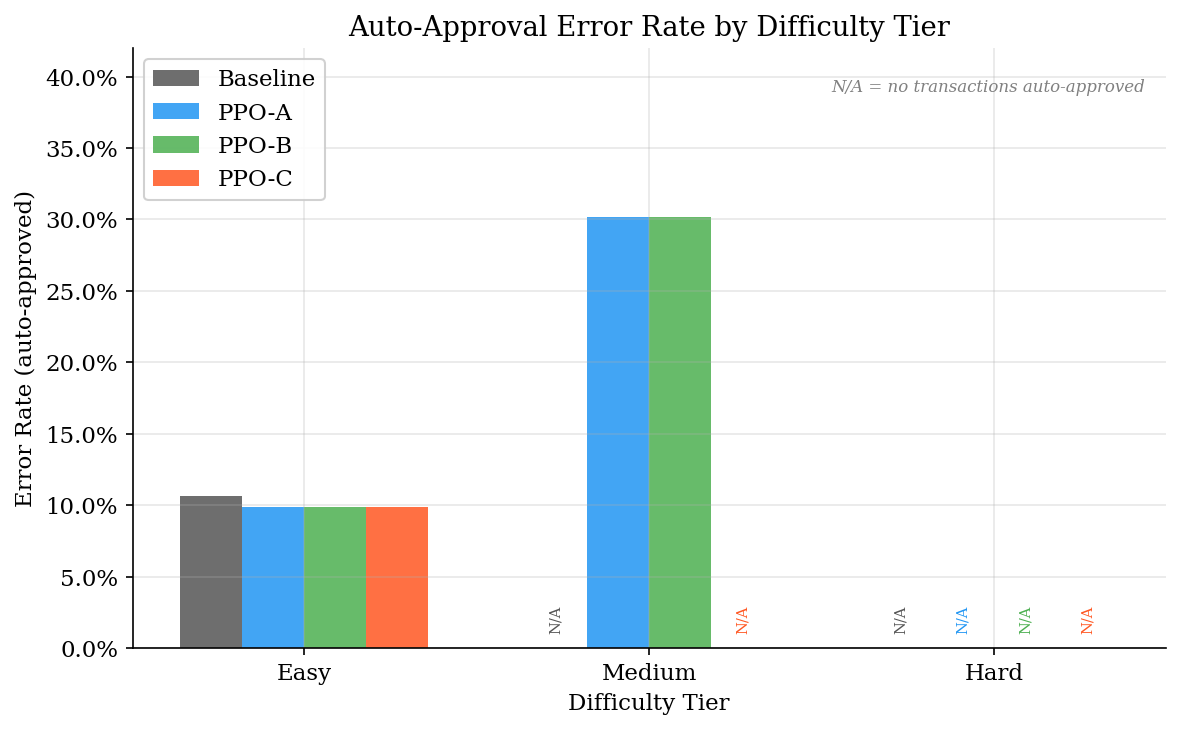
\includegraphics[width=0.78\linewidth]{fig2_error_by_tier.png}
\end{center}
\vspace{-0.15cm}

\textbf{Interpretation.}
The apparent accuracy and precision gains of PPO over the baseline are
\emph{not} statistically significant at $n{=}177$. The defensible contribution
is not "PPO improves accuracy" but "PPO learns to refuse to auto-approve the
tier where the baseline is dangerously wrong." That all three reward variants
collapse to the same policy is itself a finding: real Claude Haiku confidences
cluster at round values (0.95, 0.85, 0.75) regardless of correctness, providing
insufficient within-tier variance for reward shaping to produce different
routing behaviours. The \emph{binding constraint is confidence-score
calibration, not the RL method}. This is consistent with the broader literature
on overconfident verbally-elicited LLM confidences [Kadavath+2022, Xiong+2024].

\textbf{Next work.}
A calibration probe: re-train each variant with a well-calibrated uncertainty
signal (multi-sample self-consistency or a Platt-scaled auxiliary classifier) on
the same 705 transactions. If the three variants \emph{diverge} on calibrated
scores but \emph{converge} on raw Claude confidences, this isolates calibration
as the binding constraint rather than the RL horizon or reward design. Multi-seed
training and extension to the parent pipeline's reconciliation agent follow.

\textbf{Code, data, reproducibility.} Full code, held-out eval set, trained PPO
models, and a reproducible statistical-analysis script are at the GitHub link
above (MIT). All result numbers on this page regenerate via
\texttt{python -m agent.evaluate} followed by
\texttt{python -m experiments.statistical\_analysis}.

\end{document}
